\newcommand{\MaxBP}{\text{MaxBP}}
\newcommand{\HOBS}{\text{HOBS}}
\newcommand{\HSOBS}{\text{HSOBS}}

\section{WiMedia}

Базовая единица времени~--~суперкадр, равный $\frac{1}{16}$с. Суперкадр состоит из 256 слотов.

Устройства каждый суперкадр посылают биконы. Биконы передаются в начале суперкадра, в течение интервала времени, называемого «бикон-периодом» (BP). Бикон каждого устройства занимает фиксированный промежуток времени, называемый бикон-слотом. Первые 2 бикон-слота являются сигнальными и заполняются устройством, бикон которого занимает следующий за ими слот. Для простоты будем нумеровать слоты без учета сигнальных.

Длина бикон-периода варьирует в зависимости от количества устройств в сети. Его максимальная длина не может превосходить значения \MaxBP.

В бикон каждое устройство помимо остальной информации помещает и некую маску. Поля маски отражают состояние каждого бикон-слота с точки зрения того устройства, которое включило маску в свой бикон.

Самый старший слот, в котором находится бикон хотя бы одного устройства, будем обозначать \HOBS.

Когда устройство хочет подключиться к сети, оно выбирает бикон-слот случайным образом из окна размером R, начиная от \HOBS предыдущего шага. Если 2 устройства выбирают один и тот же слот, происходит коллизия. Другие станции это слышат и в своих биконах указывают в маске, что в данном слоте~--~шум.

\begin{figure}[h]
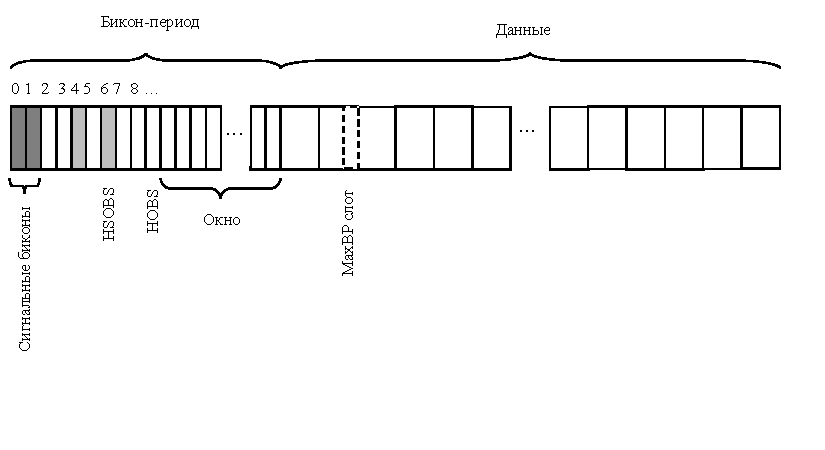
\includegraphics[width=\textwidth]{Wimedia3.pdf}
\end{figure}

Если в течение U суперкадров подряд устройство получает сигнал о бикон-коллизии, оно выбирает новый бикон-слот по описанной выше схеме.

\begin{figure}[h]
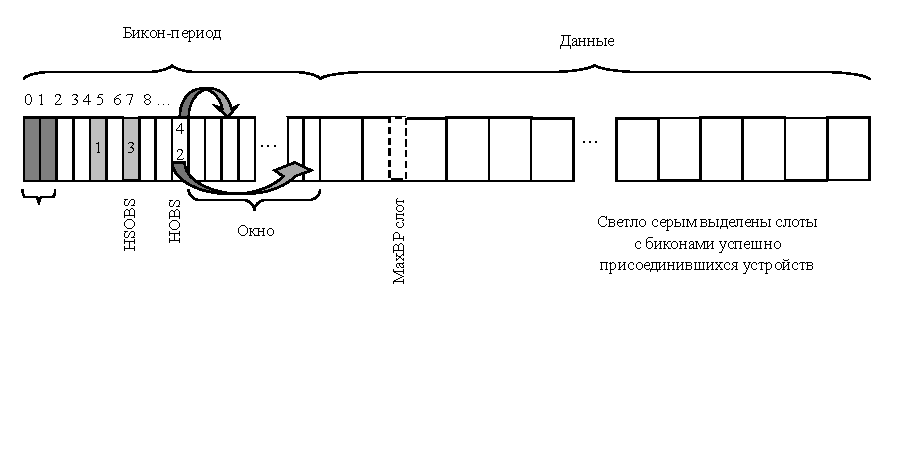
\includegraphics[width=\textwidth]{Wimedia4.pdf}
\end{figure}

Устройство, занимающее не коллизионный слот \HOBS  на протяжении последних $W \ge U+2$ суперкадров может выполнить процедуру \textbf{сжатия}~--~на следующем суперкадре переместить свой бикон в младший свободный слот.

Обозначения:
\begin{itemize}
\item $c_t$ --- количество устройств, вошедших в коллизию на очередном шаге
\item \HOBS --- старший слот, в котором находится бикон хотя бы одного устройства
\item $k$ --- количество неприсоединённых устройств
\item $\tau$ --- время, измеряемое в суперкадрах
\item $p(\tau)$ --- распределение вероятность присоединения за время $\tau$
\item \MaxBP --- максимальная длина бикон-периода
\item $M = \MaxBP - \HOBS$
\item $N$ --- всего устройств
\item $R$ --- окно, в котором станции выбирают слот для присоединения
\item $S$ --- состояние системы
\item $V(v, c)$ --- количество способов разместить $c$ биконов в $v$ слотах так, чтобы в каждом слоте было по крайней мере 2 устройства
\item $z_t = \HOBS_t - \HOBS_{t-1}$ --- максимальный номер занятого на очередном шаге слота, отчитываемый от предыдущего \HOBS
\item $\phi(S)$ --- вероятность того, что из состояния $S$ система перейдёт в успешное состояние для заданной задачи
\item $\pi(S|условие)$ --- условная вероятность того, то из состояния $S$ система за 1 шаг перейдёт в неуспешное состояние
\item $T\left\{S' \to S \right\}$ --- продолжительность шага $S'\to S$ в суперкадрах.
\end{itemize}

Задачи:
\begin{description}
\item[Задача А] найти распределение времени подключения всех $N$ устройств,
\item[Задача Б] найти распределение времени подключения произвольного заранее выбранного устройства
\end{description}

при заданной функции $R(M)$.

Допущения (Оптимистическая модель, завышает вероятность):
\begin{itemize}
\item Сжатие не происходит, пока не доходим до \MaxBP
\item После сжатия все устройства присоединяются без коллизий
\end{itemize}

Рассмотрим процесс $S = (M, k)$. Начальное состояние $S_0 = (M_0, k_0)$. Пусть сейчас мы находимся в состоянии $S' = (M', k')$.
Варианты:
\begin{itemize}
\item $\phi(S')$ --- с такой вероятностью система перейдёт в поглощающее (успешное) состояние, длительность шага -- 1 суперкадр
\item $\pi(S' |z, c)$ --- с такой вероятностью система перейдёт в состояние S, такое, что $\HOBS = \HOBS' + z$, при этом c устройств попадут в коллизии, длительность шага -- $U+1$ суперкадр. При этом $M = M' - z$; $k = c \le k'$.
\item $\pi(S'|z=M', c)$ --- с такой вероятностью будет занят последний слот и состояние будет неудачным, при этом $c$ устройств попадут в коллизии. Длительность шага $U+1+W$.
\end{itemize}

\newtheorem{wimedia1}{Утверждение}
\begin{wimedia1}
При $v > \frac{c}{2}$, $V(v, c) = 0$, в противном случае
$$ V(v,c) = v^c - \sum_{y = 1}^{v-1} C_{v}^{y} V(y, c) - \sum_{u = 1}^{v-1} C_{v}^{u} A_{c}^{u}  \sum_{y = 1}^{v-u} C_{y}^{v-u} V(y, c-u) $$
\end{wimedia1}

\begin{proof}
Первая часть утверждения очевидна. Во второй части мы из общего количества вариантов вычитаем количество вариантов, где коллизии случаются в $y < v$ слотах, а остальные слоты пустые, и затем количество вариантов размещения биконов устройств, когда $u$ слотов содержат ровно $1$ устройство.
\end{proof}

\newtheorem{wimedia2}{Утверждение}
\begin{wimedia2}
Пусть система находится в состоянии $S$ с параметрами $M$ и $k$. Тогда вероятность успеха
\begin{description}
\item[В задаче А] $\phi_A(S) = \frac{A_{k}^{R}}{R^{k}}$
\item[В задаче Б] $\phi_B(S) = \left(\frac{R-1}{R}\right)^{k-1}$
\end{description}
\end{wimedia2}

\begin{proof}
\begin{description}
\item[А] Всего возможно $R_{k}$ вариантов. Чтобы не было коллизии первое устройство может занять любой из $R$ слотов, второе – любое из $R-1$ и т. д.
\item[Б] Количество вариантов выбора слота конкретным устройством -– $R$. Остальные вольны выбирать любые слоты кроме занятого. Итого количество вариантов $R(R-1)^{k-1}$. Всех возможных вариантов снова -– $R^{k}$. После упрощения получаем искомую формулу.
\end{description}
\end{proof}

Зная $V$ можно вычислить $\pi$ и построить эволюцию процесса.

Рассмотрим пространство $(S, p,\tau)$ («состояния» + «вероятность» + «время»). Вначале состояние системы -- $S_0$, «поместим» его на гиперплоскость состояний системы, проходящую через точку временной оси $\tau_0 = 0$ (в дальнейшем будем говорить просто в точку $\tau_0 = 0$) с вероятностью $p_0 = 1$.

Пусть точке $\tau'$ временной оси соответстует $n' = n(\tau')$ состояний: $S_{\tau', 1}',...,S_{\tau', n'}'$; их вероятности $r_{\tau', 1}',...,r_{\tau', n'}'$ соответственно. Вероятность успеха при присоединении устройств в момент времени $\tau = \tau'+1: \sum_{i=1}^{n'} \phi(S_{\tau', i}')$. Таким образом, распределение принимает вид $p(\tau) = p(\tau - 1) + \sum_{i=1}^{n(\tau-1)} \phi(S_{\tau-1, i}') = \sum_{\tau' = 0}^{\tau - 1} \sum_{i = 1}^{n(\tau')} \phi(S_{\tau', i}')$

\begin{figure}[h]
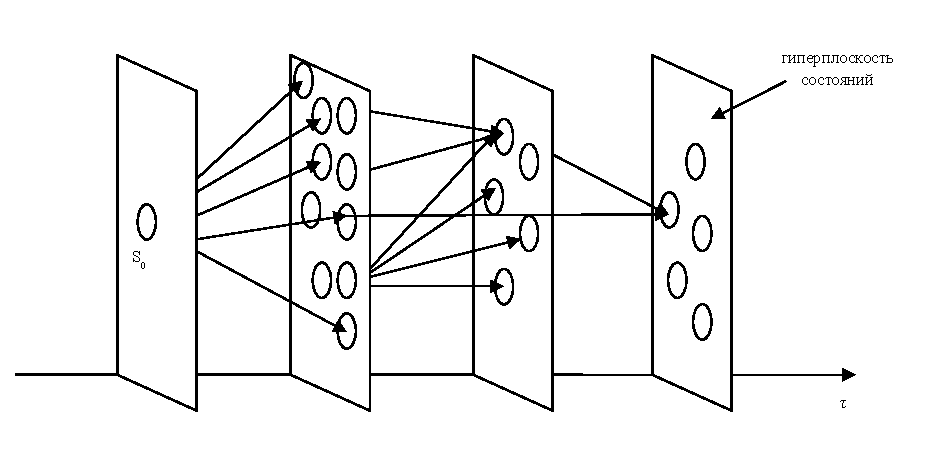
\includegraphics[width=\textwidth]{Wimedia1.pdf}
\end{figure}

Кроме того для каждого $S`$ определяем множество состояний $S$, в которые может перейти система вместе с их вероятностями $r(S)=r(S')\pi(S'|S' \to S)$. Получившиеся состояния со своими вероятностями заносятся на временную ось в моменты времени $\tau = \tau' + T$ $S' \to S$. В этой точке уже может существовать состояние $S$, в которое процесс пришел по другому маршруту. В таком случае, состояния считаются тождественными и вероятности их складываются. Благодаря этому, суммарное количество состояний не растет лавинно, хотя каждое исходное состояние и порождает много новых.

После того как момент $\tau$ обработан мы должны перейти к моменту $\tau+1$

Систему есть смысл наблюдать с шагом $U+1$.
\begin{figure}[h]
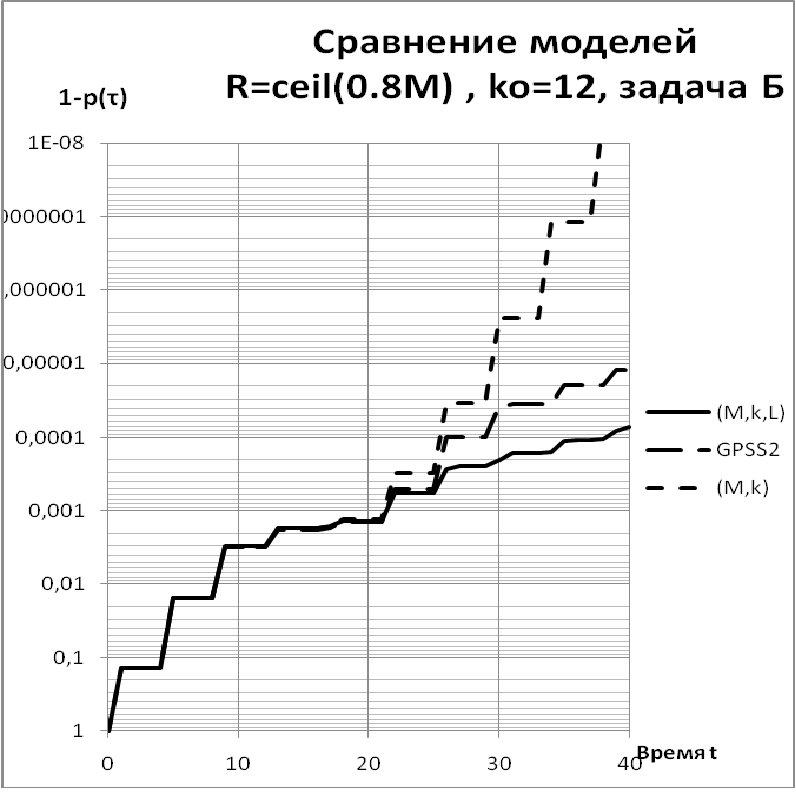
\includegraphics[width=\textwidth]{Wimedia2.pdf}
\end{figure}
